\documentclass[letterpaper]{article}

\usepackage{hw}
\usepackage{bm}
\usepackage{amsmath}
\usepackage{graphicx}
\usepackage[colorlinks=false,urlcolor=blue]{hyperref}
\usepackage{multicol}
\usepackage{paralist}
\usepackage{todonotes}
\usepackage{booktabs}
\usepackage{enumitem}
\usepackage{cleveref}
\usepackage{pdfpages}
\usepackage{fancyhdr}
\usepackage{fancyvrb}
\usepackage{tikz}
\usetikzlibrary{arrows}
\usepackage{graphicx}

\usepackage{subfig}
\DeclareCaptionType{copyrightbox}
\captionsetup{font=small}
\captionsetup{labelfont=bf}
\captionsetup[subfloat]{font=scriptsize}
\captionsetup[subfloat]{farskip=5pt}
\captionsetup[subfloat]{captionskip=1pt}
\captionsetup[table]{belowskip=0pt}

%\DeclareMathOperator*{\argmin}{arg\,min}
%\DeclareMathOperator*{\argmax}{arg\,max}

\newcommand{\email}[1]{\href{mailto:#1@cs.cmu.edu}{#1}}

\begin{document}
\title{Optimizing Matrix Operations Using Novel DRAM
  Access Primitives}
 \author{}
\date{}  
\maketitle
\begin{center}
  \textsc{\large CMU 15-745: Optimizing Compilers (Spring 2015)} \\
  \vspace{1em}
  \textsc{\large Final Report} \\
  \vspace{1em}
  \centerline{\large{Joy Arulraj (\email{jarulraj}), Anuj Kalia
    (\email{akalia})}, Jun Woo Park (\email{junwoop}) }
  \vspace{1em}
\end{center}

\section{Abstract}

Traditionally, when an application requests a set of different rows 
residing on the same memory bank, the memory access latency is 
increased due to DRAM row-buffer conflicts.
These row-buffer conflicts can be reduced by interleaving
consecutively addressed data locations across memory banks, so that
the requests are spread across different banks.
Software systems, therefore, strive hard to lay out their data structures 
to generate access patterns that can be served efficiently by 
the DRAM chips. 
For instance, DBMSs targeting analytical workloads use a columnar data 
layout so that values in the same tabular column are stored in
consecutively addressed data locations~\cite{col1}.

The design complexity of software systems can be significantly 
reduced in future DRAM chips using novel access primitives that can 
support both row and columnar access patterns efficiently. 
This is feasible by appropriately laying out the data and transforming 
the DRAM access methods.
In this project, we focussed on automatically
transforming the software access patterns to leverage these 
DRAM access primitives during compilation time.
We developed a DRAM access cost model to select the appropriate DRAM
access primitive for different patterns. We then
analyze the software access patterns in our compiler pass and then
transform the code to make use of these access primitives. 
Our evaluation of the performance impact of these transformations in 
a matrix library showed that TODO.

\section{Introduction}

DRAM access patterns significantly impact the performance of memory-bound
applications. The delay incurred while handling a cache miss is not
constant as the access latencies within DRAM are not uniform~\cite{dram1}.
DRAM is organized as a set of banks, each of which is made up of multiple
chips. Consecutive memory addresses are interleaved evenly across the
DRAM banks. Each bank has a row-buffer that is used to speed up DRAM
accesses. When the application requests for a page in a bank, the page
is first fetched into the bank's row buffer. Then, it is sent to the
the application. If the application happens to request for a page that
is already present in the row buffer, it is termed as a \textit{row-buffer
hit}. This results in the minimal DRAM access latency i.e. one memory
cycle. 
However, if the page is not present in the row buffer, then the appropriate row
in the DRAM bank needs to be activated before the requested page can be loaded into 
the row buffer and returned to the application. This event is referred to as a
\textit{row buffer miss}.

Programmers strive hard to lay out their application data structures 
to generate access patterns that can be served efficiently by the DRAM chips. 
For instance, DBMSs targeting analytical workloads use a \textit{pure-columnar} 
data layout so that values present in the same tabular column are stored 
in consecutively addressed data locations~\cite{col1,raman13,ailamaki02}. This
helps spread the DRAM accesses to multiple DRAM banks that can serve the requests in
parallel. Thus, the application can better utilize the available DRAM
bandwidth.

To give a concrete example, we compare the average time taken to compute the
sum of a row and sum of a column in a matrix laid out in row-major order.
The results are shown in ~\cref{fig:perf}. 
We observe that summing a row in this case is 2--4$\times$ faster than the
columnar sum operation.

\begin{figure*}[ht]
	\centering
	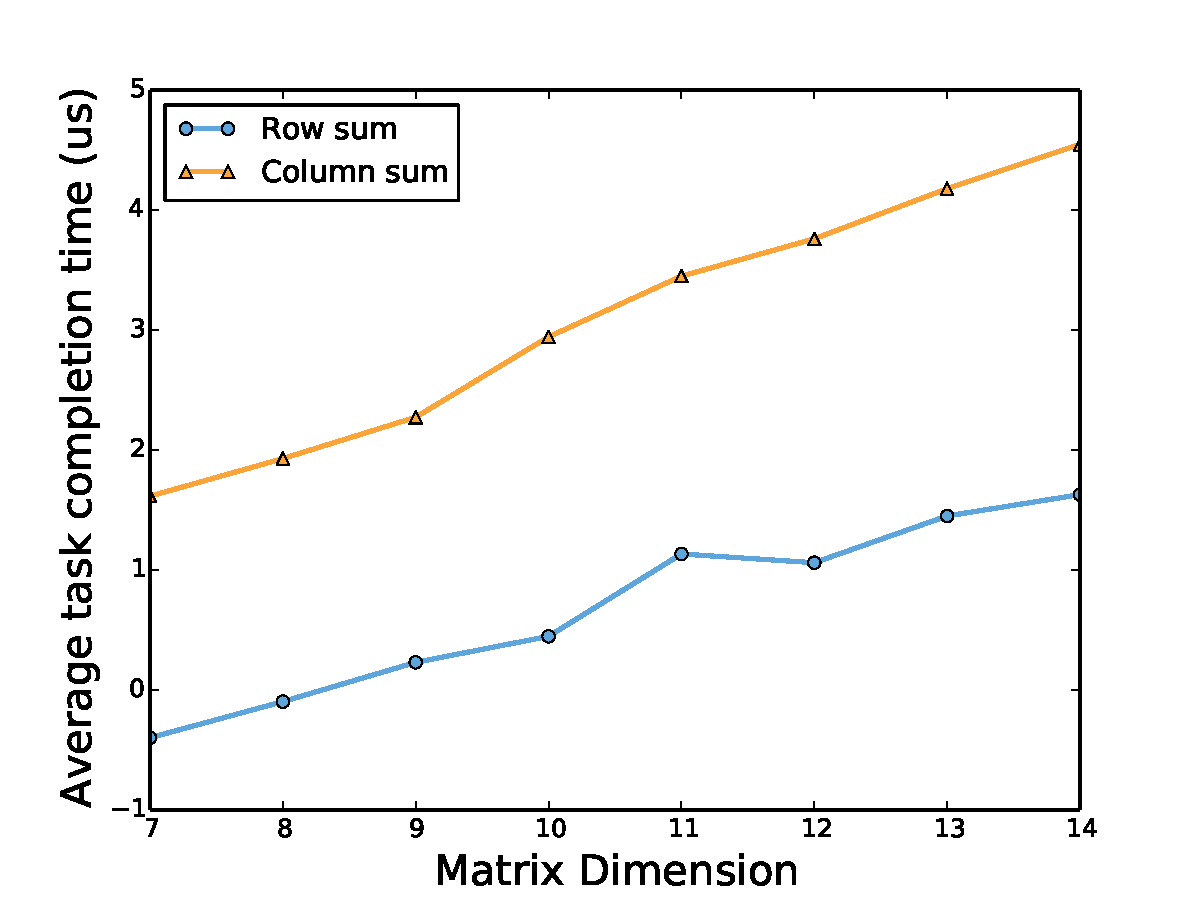
\includegraphics[scale=0.35]{images/rowmajor}
	\caption{Performance comparison of row and column oriented access patterns.
	The dimension attribute along the x-axis refers to the $\log_2$ of 
	the length of the two-dimensional square matrix. }
	\label{fig:perf}
\end{figure*}


\subsection{The Problem}

In this work, we focus on applications that have complex workloads with
mixed DRAM access patterns. For instance, in a hybrid transaction and
analytical processing (HTAP) workload~\cite{grund10}, the DBMS needs to 
access both the tuples and columns of a table efficiently. Irrespective of
whether the DBMS uses a pure-row or pure-columnar layout, one of the two
access patterns has to suffer from poor DRAM performance. For instance, assume
that the DBMS uses a pure-row layout and that the size of each tuple is one
cacheline (64 bytes). 
When serving an analytical query that needs to sum up the values in a
particular column, we need to access only that part of the tuple 
in all the tuples in the table. 
This means that we would like to access only part of a cacheline.
This is however not feasible in current hardware, as the data is laid
out in tuple-major order.  

In future hardware systems, we anticipate that we will have new DRAM access
primitives that allow us to access parts of a cacheline and not just 
entire cachelines.
These primitives will allow the application to read a cacheline 
composed of data stored in different DRAM rows by specifying 
an DRAM \textit{access pattern}. This is illustrated in ~\cref{fig:primitives}.
Consider a 4$\times$4 toy matrix. In the default row-major layout,
fetching the first column will require four DRAM read operations as
they will be serialized at the same bank. If we \textit{shuffle} 
the tile to DRAM row mapping as shown below, we observe that we can
access both the first row (cacheline 1) and first column (denoted by, say,
cacheline 1.2) using a single DRAM read operation.
This effectively allows us to retrieve the required data (for instance, a column
in a matrix) in fewer DRAM operations compared to existing DRAM access primitives. 
Therefore, we can achieve (1) lower DRAM latency, (2) more efficient DRAM
bandwidth utilization, and (3) lower energy consumption.

\begin{figure*}[ht]
	\centering
	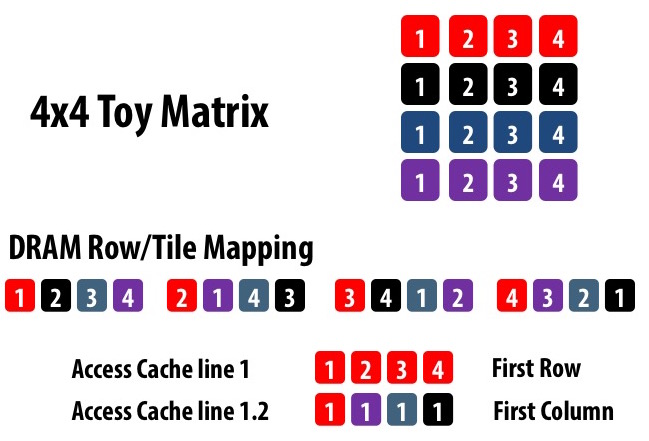
\includegraphics[width=0.8\textwidth]{images/primitives}
	\caption{Novel DRAM access primitives that allow the application to read
	both a column or a row in a small matrix in a single DRAM read operation.}
	\label{fig:primitives}
\end{figure*}


The problem we address in this work involves designing a compiler pass that 
allows us to \textit{automatically} identify the application's access
patterns and transforms the program to make use of these novel DRAM access
primitives. 
This reduces the burden on the programmer and thereby simplifies the adoption
of these DRAM access primitives.
At a high level, this involves addressing two subproblems: 

\begin{itemize}
  \item {Figuring out the different application access patterns}
  \item {Mapping the access patterns to make use of underlying DRAM access primitives.}
\end{itemize}

\subsection{Our Approach}

We have implemented an LLVM compiler pass that analyses data structure access patterns.
Currently, this targets multi-dimensional arrays of primitive data types as well as structures.
We assume that the programmer has annotated the data structures that should be
analysed using LLVM annotations.
We could apply the analysis on all loads and stores, but we wanted to restrict our
analysis to important data structures that are accessed several times in loops.
In the first stage of the pass, we parse the annotations to determine these data structures.
Then, for each loop within a function, we analyze loads and stores to these
data structures using LLVM's Scalar Evolution (SCEV) pass. Given a scope and a
register, the SCEV pass yields an expression that represents the register's
evolution inside the scope. When applied to the load or store address of the
annotated data structure in the innermost loop, this gives us the stride
with which the program performs these loads and stores.

\subsection{Related Work}

\subsection{Contributions}

We make the following contributions in this project:

\begin{itemize}
  \item {We implemented an LLVM pass that determines the different data
  structure access patterns by an application.}
  \item {We developed a basic DRAM access cost model that allows the compiler to
  map the application access pattern to the most optimal DRAM access pattern.}
  \item {We illustrate the performance benefits of these novel DRAM access primitive
  through a quantitative evaluation on different workloads in a custom matrix
  library.}
\end{itemize}

\section{Matrix Access Pattern Analysis}

\subsection{LLVM Pass}

We still plan to implement a compiler pass to perform data structure access pattern analysis, and
then do a performance evaluation to identify the impact of changing the DRAM
access pattern by using new DRAM access primitives.

The output of the compiler pass on a sample program is shown below :

We have implemented the compiler pass that analyses our benchmark library automatically without requiring
programmer annotations about stride and offset. However, we still need to figure out how to do
a realistic performance evaluation. A first-order approximation of the performance impact is
however already seen in Figure~\ref{fig:perf}. 

\begin{Verbatim}[fontsize=\small]
------------------------------
INPUT :
------------------------------
void foo(long n, long m)  {
  __attribute__((annotate(``hey, this is important''))) int A[n][m];
  struct key{
    char a;
    char b;
    char c;
  };
  __attribute__((annotate(``hey, keys''))) struct key keys[100];

  char x;
  for (long i = 0; i < n; i++) {
    for (long j = 0; j < m; j++){
      A[i][j] = 0;
      A[j][i] = 0;
      x = keys[i].a;
      keys[i].b = x;
    }
  }
}
------------------------------
OUTPUT :
------------------------------
Analysing function :: foo:
tests/a.c:i32 5           %vla = alloca i32, i32 %1, align 4    hey, this is important
tests/a.c:i32 13          %keys = alloca [100 x %struct.key], align 1   hey, keys

Inst:   store i32 0, i32* %arrayidx6, align 4
AddRec: {{0,+,(4 * %m)}<%for.cond>,+,4}<nw><%for.cond3>
ArrayRef[{0,+,1}<nuw><nsw><%for.cond>][{0,+,1}<nuw><nsw><%for.cond3>]

Inst:   store i32 0, i32* %arrayidx8, align 4
AddRec: {{0,+,4}<nuw><nsw><%for.cond>,+,(4 * %m)}<%for.cond3>
ArrayRef[{0,+,1}<nuw><nsw><%for.cond3>][{0,+,1}<nuw><nsw><%for.cond>]

Inst:   %4 = load i8* %a, align 1
AddRec: {0,+,3}<nuw><nsw><%for.cond>

Inst:   store i8 %4, i8* %b, align 1
AddRec: {1,+,3}<nw><%for.cond>
\end{Verbatim}

We are now figuring out how best to use this information to automatically
choose the best data access and layout pattern.

\subsection{DRAM Access Cost Model}

\begin{figure*}[ht!]
	\centering
	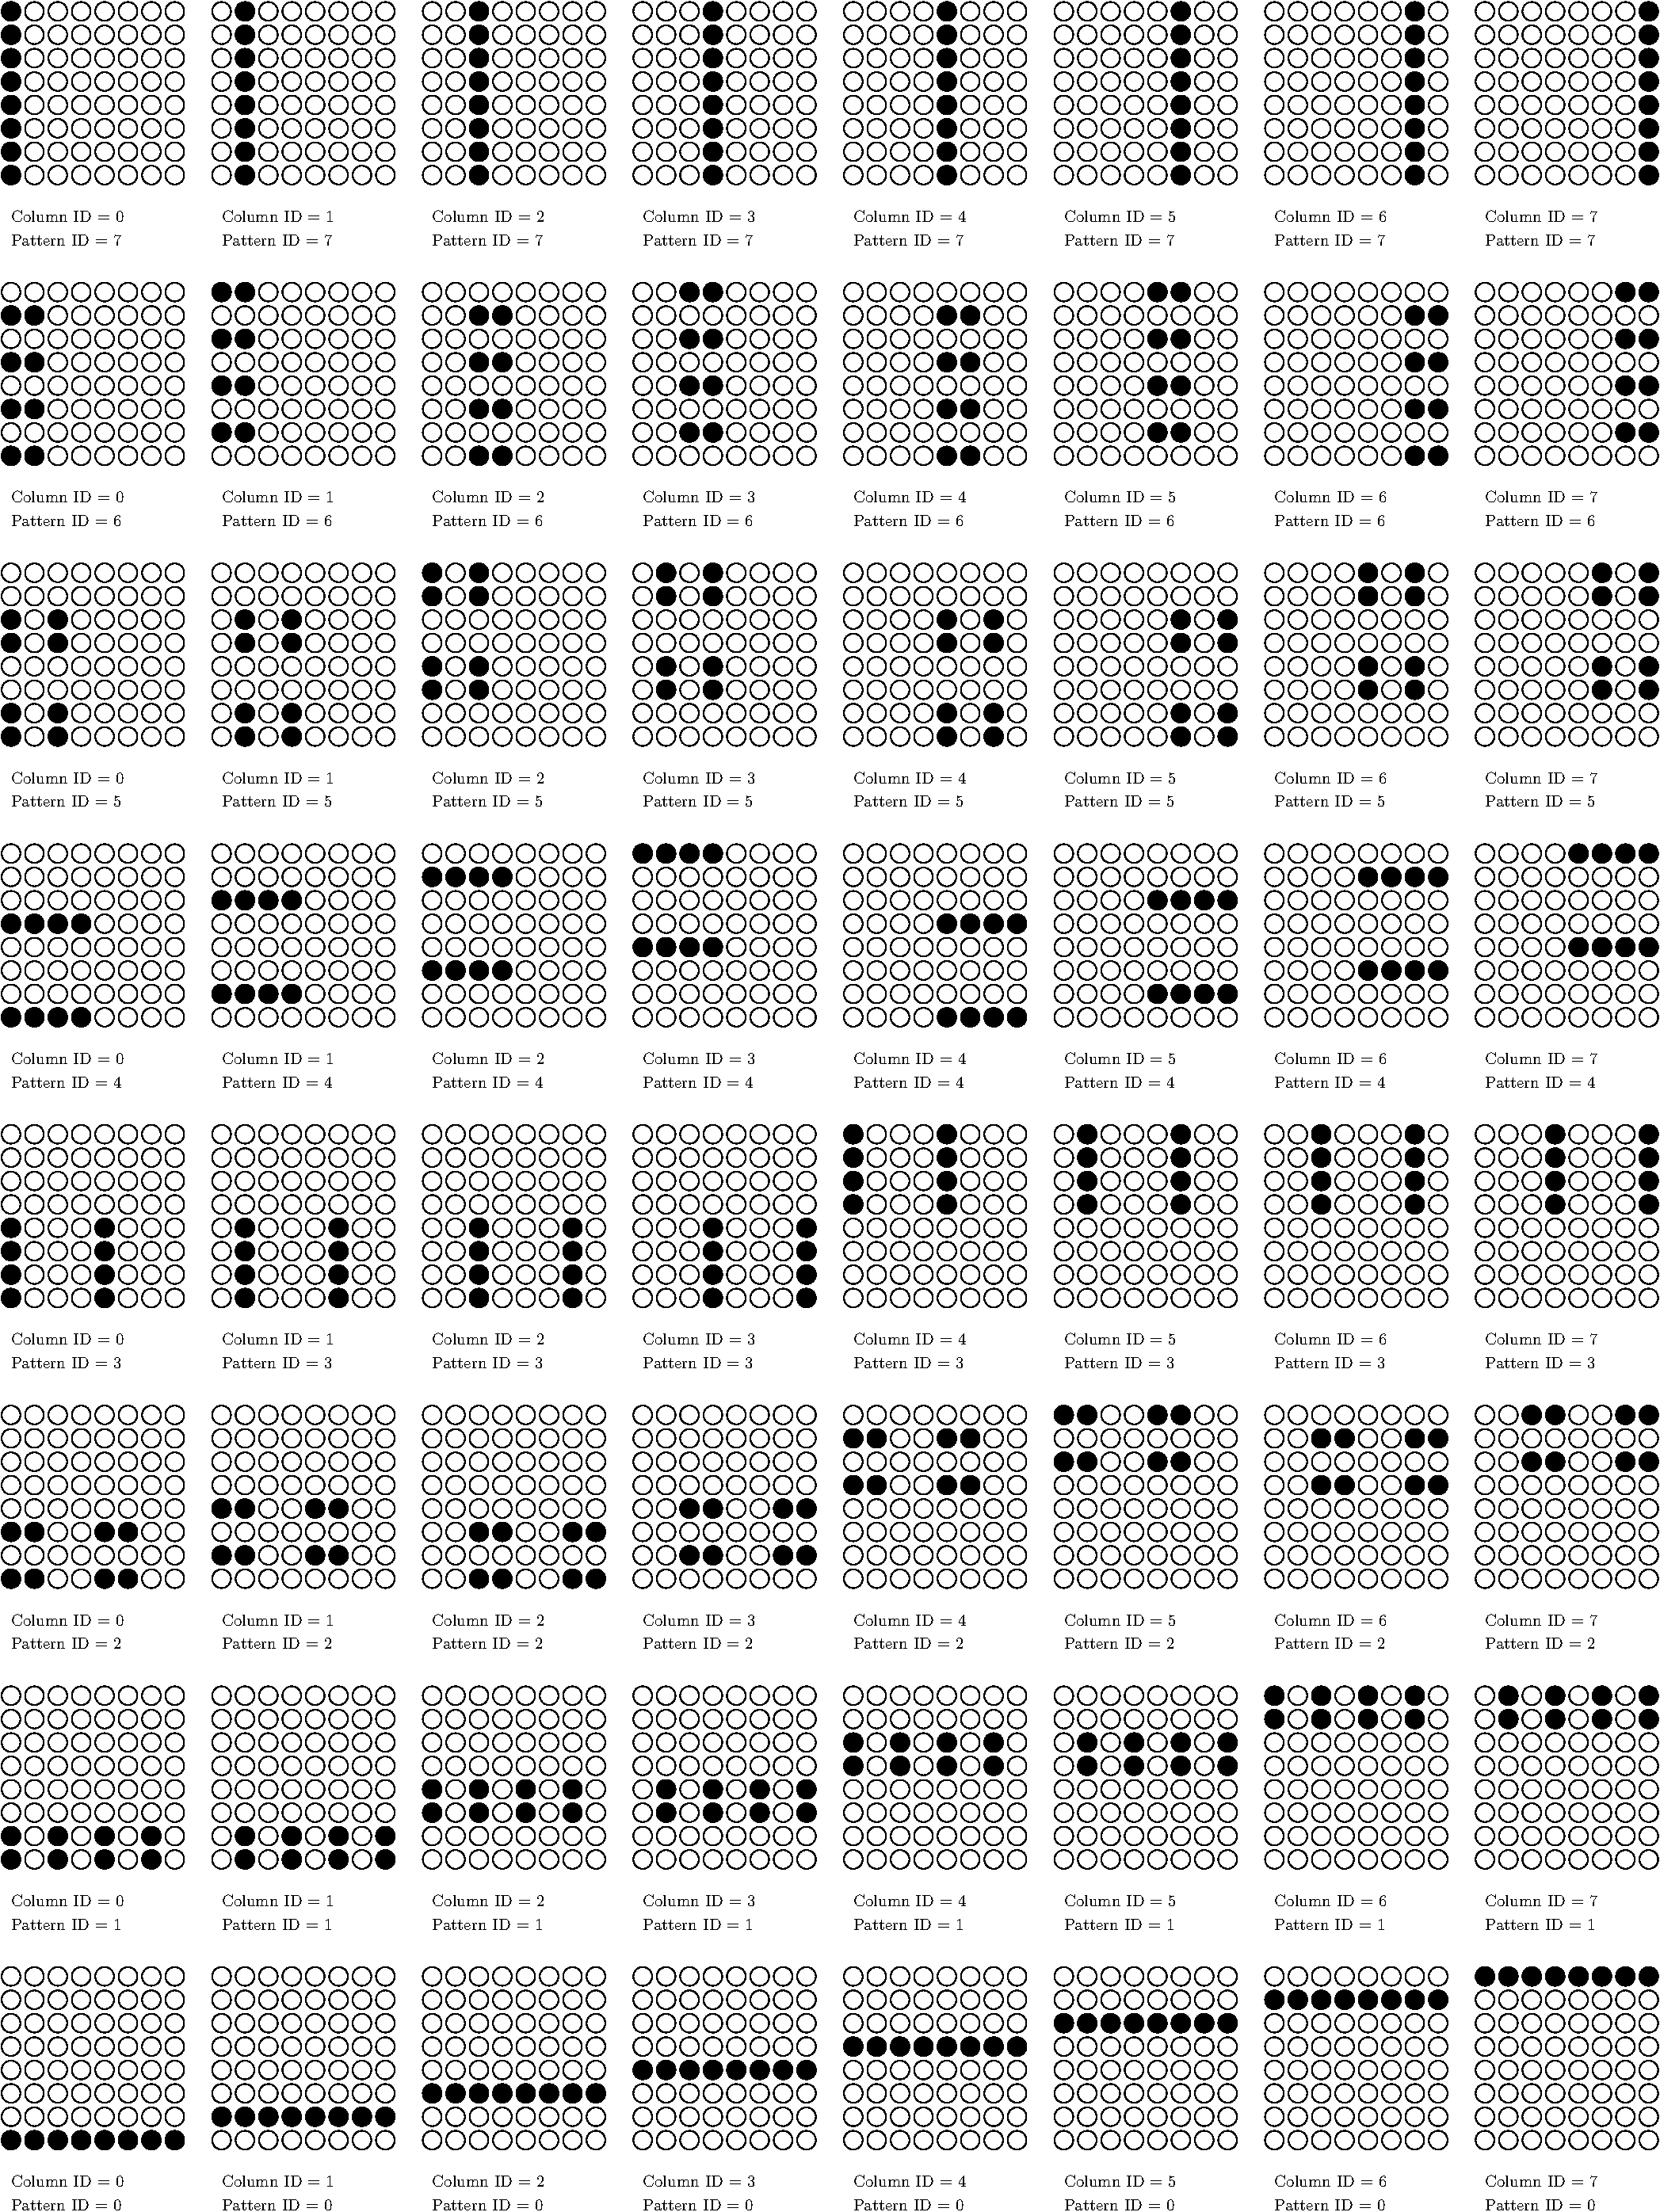
\includegraphics[width=0.9\textwidth]{images/pattern}
	\caption{List of possible patterns for a 8x8 matrix with a given shuffling
	function. There are 64 patterns and the column id refers to the cacheline
	being accessed. The elements of the cacheline returned are highlighted.}
	\label{fig:pattern}
\end{figure*}

\section{Experimental Setup}

\section{Experimental Evaluation}

\begin{figure*}[t]
    \centering
    \subfloat[64$\times$64 tiles]{
	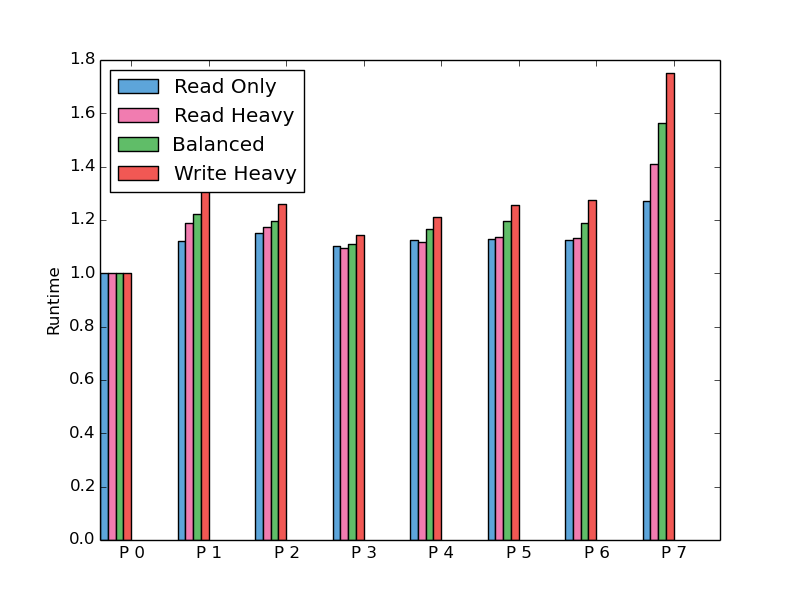
\includegraphics[width=0.5\textwidth]{images/64_runtime}
    } 
    \subfloat[128$\times$128 tiless]{
	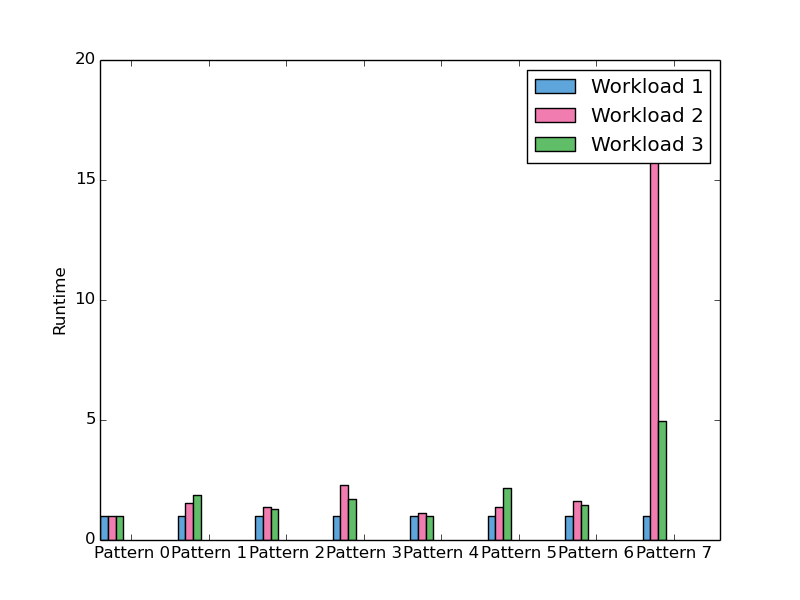
\includegraphics[width=0.5\textwidth]{images/128_runtime}
    }\\
    \subfloat[256$\times$256 tiles]{
	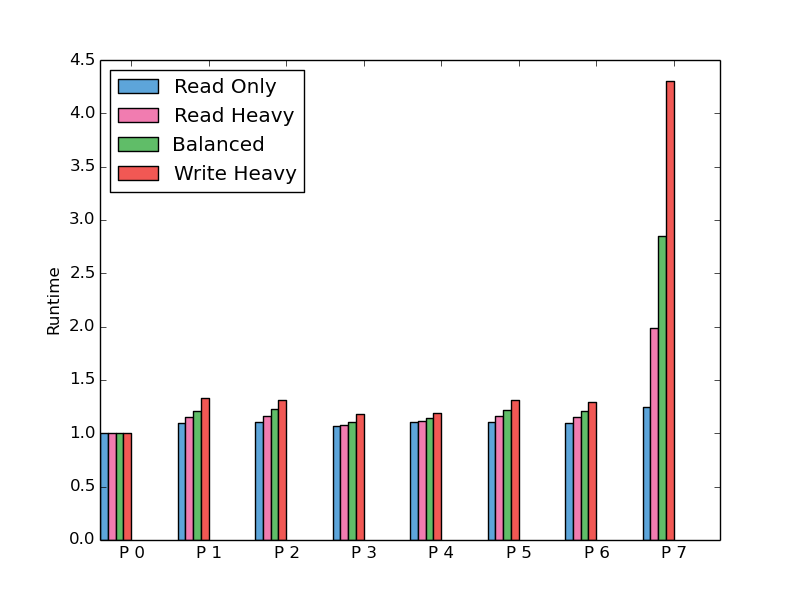
\includegraphics[width=0.5\textwidth]{images/256_runtime}
    } 
    \subfloat[512$\times$512 tiless]{
	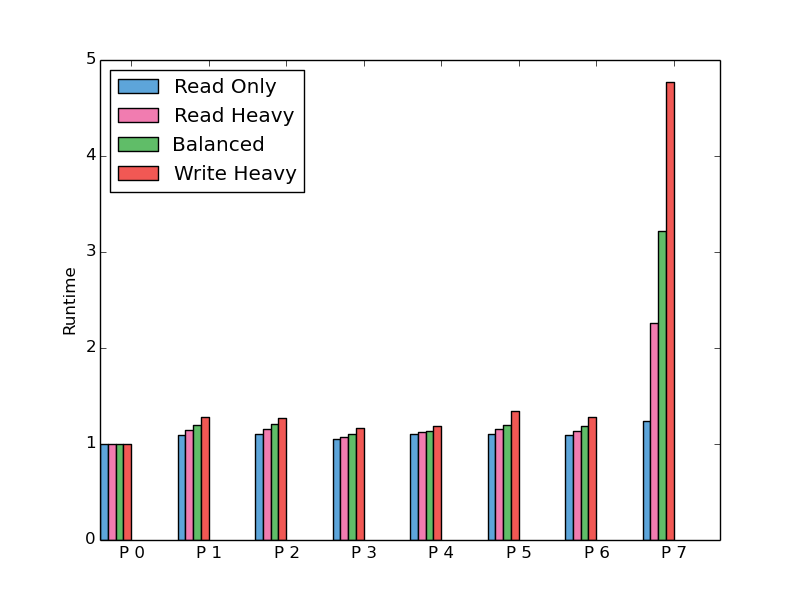
\includegraphics[width=0.5\textwidth]{images/512_runtime}
    }
    \caption{\textbf{Performance -- Evaluation of workload}}
        
    \label{fig:evaluation}
\end{figure*}

\section{Surprises and Lessons Learned}

We were pleasantly surprised by the support in LLVM for analysing scalar expressions and annotations.
This helped reduce the complexity of the compiler pass.

\section{Conclusions and Future Work}

\section{Distribution of Total Credit}

\bibliographystyle{acm}
\bibliography{ref}

\end{document}

%%% Local Variables:
%%% mode: latex
%%% TeX-master: "."
%%% End:
